\chapter{Elementi Costitutivi}\label{cap:Hardware}

\begin{minipage}{12cm}\textit{
		In questo capitolo si vogliono descrivere e caratterizzare i 3 elementi salienti dell'esperimento:
		\begin{enumerate}
			\item \nameref{TrasformatoreModelloTokamak}
			\item \nameref{CurrentSense}
			\item \nameref{CurrentDriver}
		\end{enumerate}
	}
	Essi verranno analizzati al fine di mettere in luce i loro punti di forza, ovvero i motivi che hanno portato alla loro scelta, e si evidenzieranno eventuali problemi che affliggono in componenti, problemi di cui si è tenuto conto nello sviluppo del progetto per poterli annullare e/o compensare. 
\end{minipage}

\newpage

\section{Trasformatore, un Modello di Tokamak}\label{TrasformatoreModelloTokamak}

Come visto nell'introduzione, la tesi ha come obiettivo la prototipazione del sistema di controllo per le bobine magnetiche presenti in impianti tokamak.
\begin{figure}[H]
	\centering
	\caption[Schema interno di un Tokamak]{Interno Tokamak}
	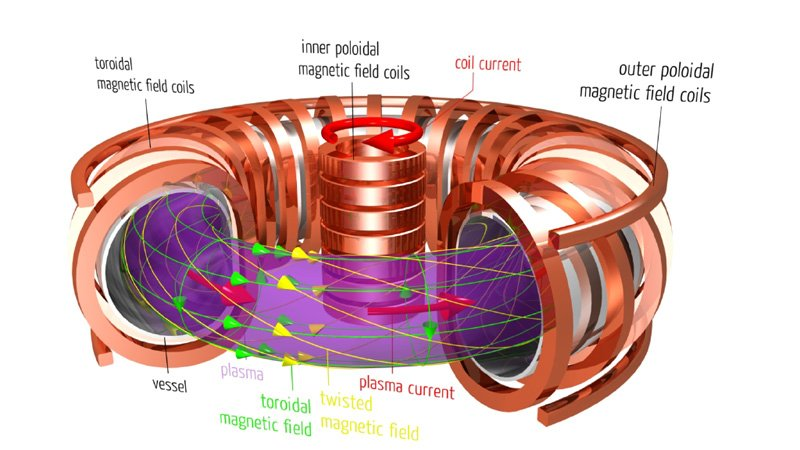
\includegraphics[width=1\textwidth]{Trasformatore/tokamak_scheme.jpg}
\end{figure}
\noindent
Le bobine (poloidali e toroidali) servono a controllare il Plasma presente nel \textit{Vessel} dell'impianto e confinare il Plasma all'interno di un flusso compresso dentro la camera, le alte temperature e la forte compressione a cui è sottoposto il Plasma, permette di realizzare eventi di \textbf{Fusione Nucleare Controllata} tra gli atomi di idrogeno che compongono il Plasma usato dentro il Tokamak.\\
Essendo però impossibile usare in un ambiente controllato un vero Tokamak, specie in un laboratorio universitario, si è usato un sistema fisico equivalente per ricreare l'interazione tra le \textbf{Bobine e il Plasma}.\\
Il modello equivalente in questione è quello di \textbf{Trasformatore Elettrico} nella relazione \textit{Primario-Secondario} (con ovviamente alcune approssimazioni e la semplificazione di varie \nonLinearita sui suoi parametri, a delle costanti).\\
Grazie a questa similitudine è stato possibile replicare in sicurezza la fisica presente all'interno di un Tokamak, nell'ambiente controllato del laboratorio usando una batteria in grado di erogare molti Ampere come fonte di alimentazione dell'esperimento.\\

\subsection{Richiami di elettronica}
Prima di modellare ed analizzare l'esperimento della tesi, è necessario richiamare qualche proprietà/concetto di elettronica per poter comprendere i passaggi matematici e fisici:
\vspace{-5mm}
\NumTabs{7}
\begin{itemize}[itemsep=-4mm]
	\item \nameref{th:KirchhoffNodi}
	\item \nameref{th:KirchhoffMaglie}
	\item \nameref{def:induttoreIdeale}
	\item \nameref{def:induttanza}
	\item \nameref{def:trasformatoreIdeale}
\end{itemize}


\begin{teorema}[Prima legge di Kirchhoff (legge dei nodi)\label{th:KirchhoffNodi}]
	La somma algebrica delle intensità di corrente nei rami facenti capo allo stesso nodo è nulla.
	\begin{empheq}[box=\mathResult]{equation} \label{eq:KirchhoffNodi}
		\sum I_k = 0
	\end{empheq}
\end{teorema}

\begin{teorema}[Seconda legge di Kirchhoff (legge delle maglie)\label{th:KirchhoffMaglie}]
	La somma algebrica delle f.e.m. (Forze Elettro Motrici) agenti lungo i rami di una maglia è uguale alla somma algebrica dei prodotti delle intensità di corrente di ramo per le rispettive resistenze (del ramo).
	\begin{empheq}[box=\mathResult]{equation} \label{eq:KirchhoffMaglie}
		\sum_{\forall k} V_k = \sum_{\forall k} f_{em_k}
	\end{empheq}
\end{teorema}
\vspace{-3mm}
\noindent
Oltre ai teoremi di Kirchhoff, che ci serviranno per ricavare le equazioni della dinamica, enunciamo ora le proprietà degli induttori, indispensabili per poter parametrizzare il Trasformatore.

\begin{de}[Induttore Ideale\label{def:induttoreIdeale}]
	Un \textit{Induttore Ideale} si oppone \underline{solo} alle variazioni di corrente, variando la tensione ai suoi capi di conseguenza, non presenta nessuna resistenza elettrica in caso di correnti costanti ai suoi capi.\\
	Il suo valore è detto \textbf{coefficiente di autoinduzione}, tipicamente espresso con il simbolo $L$, la cui unità di è l'Henry [$H$].\\
	Un Induttore accumula energia all'interno di un campo magnetico, e questa relazione è descritta dall'equazione:
	\begin{vwcol}[widths={0.4,0.6}, sep=8mm, rule=0px]
		\vspace{-3mm}
		\begin{empheq}[box=\mathStep]{equation} \label{eq:flussoMagnetico}
			\Phi _{B}=Li
		\end{empheq}
		\newpage % con wcol, le colonne sono "pagine"
		\hfill\\[-2mm]
		$ \Phi _{B} $ := \textbf{Flusso magnetico}\\
		$L$ := \textbf{Coefficiente di autoinduzione}
	\end{vwcol}
	\noindent
	Applicando la legge di Faraday (ignorando momentaneamente la conservazione dell'energia, ovvero la legge di Lenz) alla circuitazione del circuito costituito dalla sola induttanza, si ottiene:
	\begin{vwcol}[widths={0.4,0.6}, sep=8mm, rule=0px]
		\vspace{-3mm}
		\begin{empheq}[box=\mathStep]{equation}
			V = \frac {d\Phi _{B}}{dt}
		\end{empheq}
		\newpage % con wcol, le colonne sono "pagine"
		\hfill\break \hfill\\[-2mm]
		$ V $ := \textbf{Potenziale indotto} ai morsetti del circuito
	\end{vwcol}
	\noindent
	Derivando ora l'equazione \ref{eq:flussoMagnetico} ad entrambi i membri rispetto al tempo, si ottiene:
	\begin{empheq}[box=\mathStep]{equation}
		\displaystyle \frac {d\Phi _{B}}{dt}=L{\frac  {di}{dt}}+i{\frac  {dL}{dt}}
	\end{empheq}
	In molti casi fisici, però, l'induttanza può essere considerata costante rispetto al tempo (o tempo-invariante), da cui la formula che useremo risulta pari a:
	\begin{empheq}[box=\mathStep]{equation}
		\displaystyle {\frac {d\Phi _{B}}{dt}}=L{\frac {di}{dt}}
	\end{empheq}
	Combinando le equazioni precedenti si ottengono quindi i legami ingresso uscita rispetto alla tensione e alla corrente:
	\begin{empheq}[box=\mathCalc]{equation}
		{\displaystyle V(t)={L{\frac {di(t)}{dt}}}} \Leftrightarrow i(t) = \frac{1}{L} \int V(t) dt
	\end{empheq}
\end{de}
\noindent
Nel calcolo della \ref{eq:flussoMagnetico}, abbiamo omesso la legge di Lenz, poichè per parametrizzare l'induttore il segno '$ - $' complica inutilmente i calcoli essendo in realtà assegnato dalla polarizzazione del circuito mentre si svolgono i calcoli.\\
La legge di Lenze prende molta importanza invece durante il fenomeno dell'\textbf{Induttanza}, ovvero quando 2 induttori vengono collegati tra loro per mezzo di un campo magnetico:
\begin{de} [Induttanza\label{def:induttanza}]
	L'induttanza è la proprietà dei circuiti elettrici tale per cui la corrente (intesa variabile nel tempo) che li attraversa induce una \textbf{Forza ElettroMotrice} (f.e.m.) \textit{Indotta} che si oppone alla variazione di corrente (legge di Lenz).\\
	In questi scenari (vedi Trasformatore Elettrico ad esempio), 2 ciruiti sono accoppiati magneticamente tra di loro attraverso 2 induttori, si ottiene quindi che, la variazione del flusso magnetico da parte del primo induttore, crea una \textbf{Forza ElettroMotrice} (f.e.m.) \textit{indotta} contraria nell'altro circuito:
	\begin{vwcol}[widths={0.4,0.6}, sep=8mm, rule=0px]
		\vspace{-3mm}
		\begin{empheq}[box=\mathCalc]{equation}
			{\displaystyle -{\frac {d\Phi _{B}}{dt}}={\mathcal {E}}=V}
		\end{empheq}
		\newpage % con wcol, le colonne sono "pagine"
		\hfill\break \hfill\\[2mm]
		$ \mathcal{E} $ := \textbf{Forza ElettroMotrice} (f.e.m.) indotta
	\end{vwcol}
\end{de}
\noindent
Per concludere uniamo insieme i concetti di \nameref{def:induttoreIdeale} e \nameref{def:induttanza} così da ottenere la descrizione matematica di un Trasformatore Monofase Ideale (\cite{Transformatore}\footnote{Senso di misura del secondario opposto nell'articolo a quello presentato nella tesi}):
\begin{figure}[H]
	\centering
	\caption[Trasformatore ideale con Campo magnetico]{Trasformatore Ideale}
	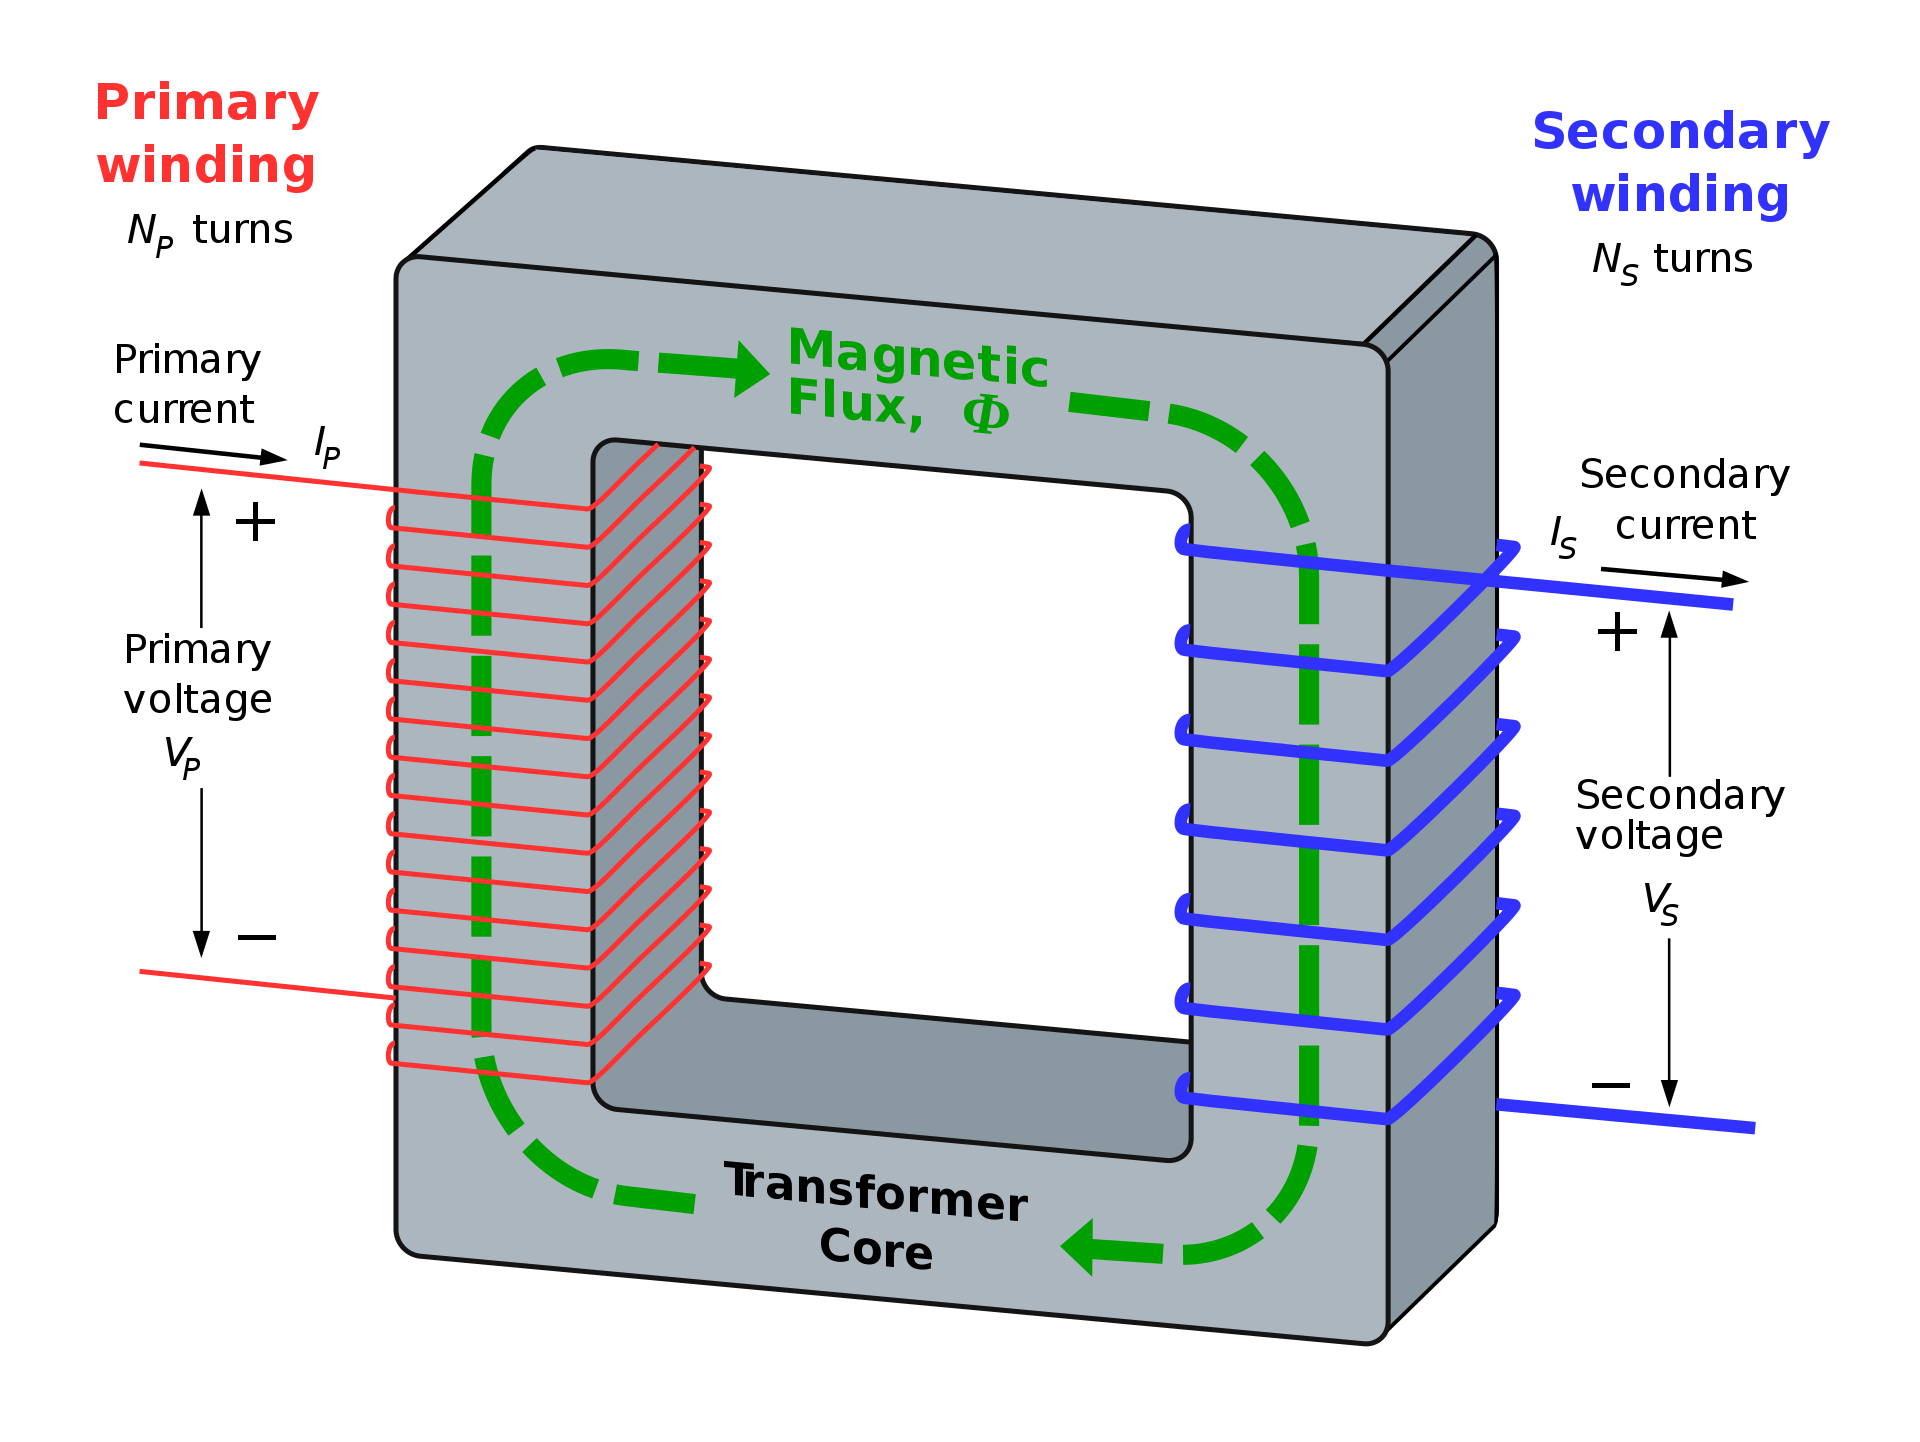
\includegraphics[width=0.8\textwidth]{Trasformatore/trasformatore.png}
\end{figure}

\begin{de}[Trasformatore Ideale Monofase\label{def:trasformatoreIdeale}]
	Il Trasformatore è una macchina elettrica, basata sul fenomeno dell'induzione elettromagnetica, il cui scopo è trasformare tra il circuito primario (ingresso) e il circuito secondario (uscita) la tensione e corrente in ingresso in un altra scala mantenendo inalterata la potenza elettrica.\\
	Permette quindi il trasferimento per mezzo magnetico, di energia tra 2 circuiti fisicamente disaccoppiati, accoppiandoli induttivamente.
	
	In un Trasformatore il circuito Primario e il Secondario condividono lo stesso campo magnetico, e conseguentemente lo stesso flusso $\Phi _{B}$.\\
	Nel caso ideale, quindi, si ha che:
	\begin{vwcol}[widths={0.4,0.6}, sep=8mm, rule=0px]
		\vspace{-3mm}
		\begin{empheq}[box=\mathStep]{equation}
			\Phi_{B} = \Phi_{B_P} - \Phi_{B_S}
		\end{empheq}
		\newpage % con wcol, le colonne sono "pagine"
		\hfill\break \hfill\\[-2mm]\noindent
		{\footnotesize
			Il '$ - $'  tra i campi magnetici è dovuto al verso delle correnti\\
			che creano 2 campi magnetici tra loro contrapposti
		}
	\end{vwcol}
	\noindent
	Siccome tale flusso varia nel tempo, induce nei due avvolgimenti delle f.e.m. (vedi \nameref{def:induttanza}):
	\begin{empheq}[box=\mathStep]{equation}
		e_p = N_1 \frac{d \Phi_{B}}{dt} ; e_s = -N_2 \frac{d \Phi_{B}}{dt}
	\end{empheq}
	I segni non sono entrambi concordi a causa del verso del flusso, che nel primario è concorde e nel secondario discorde (e qui torna la forza di Lenz).\\
	Viste dai morsetti del trasformatore, abbiamo che le tensioni istantanee (dovute alle correnti presenti nei 2 rami) sono pari a:
	\begin{empheq}[box=\mathCalc]{equation} \label{eq:tensioneTrasformatore}
		\displaystyle \left \{ \begin{array}{l}
			V_{P} = R_P I_P + L_{PP} \dot I_P - L_{SP} \dot I_S \\
			V_{S} = R_S I_S - L_{PS} \dot I_P + L_{SS} \dot I_S \\
		\end{array}
		\right.
	\end{empheq}
	Dove $R_P$ e $R_S$ rappresentano le resistenze equivalenti viste dai morsetti (i carichi).\\
	Con i coefficienti di mutua induttanza che si ricavano dalla Def di \nameref{def:induttoreIdeale}:
	
	\begin{center}
		\begin{tabular}[t]{c c}
			$ \displaystyle L_{pp} = \frac{N_P  \Phi_{B_P} }{i_P} $ & $ \displaystyle L_{ps} = \frac{N_S  \Phi_{B_P} }{i_P} $ \\[5mm]
			$ \displaystyle L_{sp} = \frac{N_P  \Phi_{B_S} }{i_S} $ & $ \displaystyle L_{ps} = \frac{N_S  \Phi_{B_S} }{i_S} $
		\end{tabular}
	\end{center}
\end{de}

\noindent
Arrivati a questo punto abbiamo gli strumenti necessari per poter modellare matematicamente l'esperimento in esame nella tesi.
\newpage

\subsection{Modellazione Fisica} \label{subsec:ModelloFisico}
Usando i concetti esposti, vediamo ora una buona approssimazione, passante per un modello lineare a parametri costanti della dinamica tra \textbf{Bobina e Plasma}.\\
Come descritto nell'articolo di \cite{TokamakCircuit}, è possibile modellare la dinamica \textbf{Bobina - Plasma} come fosse il circuito di un
\nameref{def:trasformatoreIdeale}:
\begin{figure}[H]
	\centering
	\caption[Circuito Equivalente Bobina/Plasma all'interno di un Tokamak]{Circuito Equivalente Bobina/Plasma}
	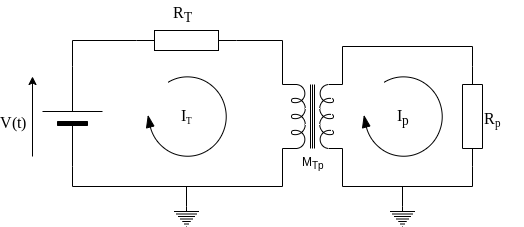
\includegraphics[width=1\textwidth]{Trasformatore/PlasmaCircuit-PlasmaCircuit.png}
\end{figure}
\NumTabs{11}
\begin{leg}
	\item $V(t)$\tab:= Tensione di controllo della Corrente $I_T$
	\item $I_T$\tab:= Corrente del Trasformatore
	\item $R_T$\tab:= Resistenza equivalente Trasformatore
	\item $I_p$\tab:= Corrente di Plasma
	\item $R_p$\tab:= Resistenza di Plasma
	\item $M_{Tp}$\tab:= Coefficiente di Induttanza Trasformatore $\rightarrow$ Plasma
\end{leg}
\paragraph{Difformità dalla realtà} Nella realtà $R_p$ e $M_{Tp}$ sono dei parametri che variano in funzione dello stato del Plasma (Temperatura, Energia, Evoluzione dell'esperimento, ecc\ldots), ma per ovvie ragioni di difficoltà nel riprodurre in laboratorio simili \nonLinearita, noi prenderemo per costanti questi parametri.

\subsection{Semplificazione Primario - Secondario}
Sempre dallo stesso articolo di \cite{TokamakCircuit}, si evince che è possibile modellare questa relazione tra i 2 circuiti prendendo in considerazione \textbf{solo} le forze di induzione dovute alla corrente che il Primario trasferisce sul Secondario, ciò permette di semplificare ulteriormente il circuito trascurando le correnti indotte dal Plasma dentro la Bobina del Primario.\\
Usando queste osservazioni si ottiene quindi il circuito equivalente:
\begin{figure}[H]	\label{fig:PlasmaSemplificato}
	\centering
	\caption[Circuito Semplificato Bobina/Plasma]{Circuito equivalente Bobina/Plasma semplificato}
	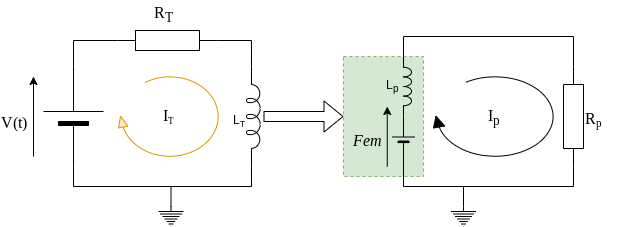
\includegraphics[width=1\textwidth]{Trasformatore/PlasmaCircuit-EquivalentCalc.png}
\end{figure}

\NumTabs{11}
\begin{leg}
	\item $V(t)$\tab:= Tensione di controllo della corrente $I_T$
	\item $I_T$\tab:= Corrente del Trasformatore
	\item $R_T$\tab:= Resistenza equivalente Trasformatore
	\item $I_p$\tab:= Corrente di Plasma
	\item $R_p$\tab:= Resistenza di Plasma
	\item $M_{Tp}$\tab:= Coefficiente di Induttanza Trasformatore $\rightarrow$ Plasma
	\begin{itemize} [topsep=-1mm,itemsep=0mm,label=$ \circ $]
		\item $L_T$\tab:= Induttanza equivalente Trasformatore
		\item $L_p$\tab:= Induttanza equivalente Plasma
	\end{itemize}
\end{leg}
\noindent
Usando questa semplificazione dall'equazione \ref{eq:tensioneTrasformatore} del trasformatore ignoriamo che la tensione sul Primario è influenzata dal Secondario; in questa condizione il circuito del Primario evolve come sistema indipendente rispetto al Secondario, e la sua evoluzione influenza il Secondario senza risentirne.

\newpage
\subsection{Dal circuito alla dinamica}\label{subsec:dinamicaCircuito}
Analizziamo ora la dinamica del circuito semplificato \ref{fig:PlasmaSemplificato} analizzando le 2 maglie del circuito:
\subsubsection{Dinamica di Plasma}
\vspace{-2mm}
Per calcolare la dinamica della corrente di Plasma usando la \nameref{th:KirchhoffMaglie} sulla maglia del secondario:
\begin{empheq}[box=\mathStep]{equation*}
	F_{em} = L_p \dot I_p + I_p R_p
\end{empheq}
Grazie al principio dell'\nameref{def:induttanza} siamo in grado di risalire al termine generatrice della $F_{em}$: 
\begin{empheq}[box=\mathStep]{equation*}
	F_{em} = -M_{Tp} \dot I_T
\end{empheq}
Perciò, unendo insieme i blocchi otteniamo:
\begin{vwcol}[widths={0.6,0.4}, sep=5mm, rule=0px]
	\vspace{-3mm}
	\begin{empheq}[box=\mathCalc]{equation} \label{eq:correntePlasmaDinamica}
		-M_{Tp} \dot I_T = L_p \dot I_p + I_p R_p
	\end{empheq}
	\newpage % con wcol, le colonne sono "pagine"
	\hfill\\[-1mm]\noindent
	\begin{spacing}{1.25}
		{\footnotesize
			Da notare la somiglianza con\\
			l'equazione del trasformatore \ref{eq:tensioneTrasformatore}
		}
	\end{spacing}
\end{vwcol}\vspace{-3mm}
\noindent
\begin{oss}
	Dalla eq \ref{eq:correntePlasmaDinamica} è interessante notare che rendere la corrente di Plasma costante, equivale a fissare una $F_{em}$ di costante.\\
	In un Tokamak reale, anche se l'obiettivo è controllare la corrente di Plasma, misurarla direttamente risulta essere problematico, a tale scopo nei Tokamak reali, viene usata la \textbf{Tensione di Loop} (\cite{MagneticDiagnostics}) come indicatore della $ I_p $, che nel nostro caso coincide esattamente con la $ F_{em} $ del secondario (problematica discussa in seguito, vedi \nameref{sub:parametriMisurati}).
\end{oss}


\subsubsection{Dinamica del Trasformatore}
\vspace{-3mm}
Vediamo ora la dinamica della corrente del Trasformatore, in funzione della \textit{Tensione di controllo}.\\
Il calcolo avviene seguendo gli stessi procedimenti della corrente di Plasma, usando sempre il \nameref{th:KirchhoffMaglie}, e si ottiene come equazione di maglia:
\begin{empheq}[box=\mathCalc]{equation} \label{eq:correnteTrasformatoreDinamica}
	V(t) = L_T \dot I_T + I_T R_T
\end{empheq}

\subsection{Funzione di Trasferimento}
Nella sezione "\nameref{subsec:dinamicaCircuito}" abbiamo ottenuto la dinamica istantanea dei 2 rami del circuito \ref{fig:PlasmaSemplificato}.\\
Vogliamo ora ricavare le funzioni di trasferimento dei 2 rami e trovare così la funzione di trasferimento Ingresso uscita del Trasformatore.
\subsubsection{Funzione di Trasferimento Plasma}
\vspace{-3mm}
Volendo calcolare la funzione di trasferimento per le dinamiche forzate, partiamo dall'equazione \ref{eq:correntePlasmaDinamica} risolvendola per condizioni iniziali nulle.
\begin{center}
	{\large
		$ s I_p L_p  + I_p R_p = -s I_T M_{Tp} \Rightarrow I_p( s L_p + R_p) = -s I_T M_{Tp} \Rightarrow$ \\ 
		$ I_p(s) = \frac{-s M_{Tp}}{( s L_p + R_p)} I_T(s) $
	}
\end{center}
\noindent
Arrivando così a scrivere come funzione di trasferimento per il Plasma (Secondario):
\begin{empheq}[box=\mathCalc]{equation} \label{eq:correntePlasmaLaplace}
	\frac{I_p(s)}{I_T(s)}  = \frac{-s M_{Tp}}{( s L_p + R_p)}
\end{empheq}

\subsubsection{Funzione di Trasferimento Trasformatore}
\vspace{-5mm}
Similmente a quanto fatto per Plasma, partendo dall'equazione \ref{eq:correnteTrasformatoreDinamica} in condizioni iniziali nulle abbiamo:
\begin{center}
	{\large
		$ s I_T L_T  + I_T R_T = V(s) \Rightarrow I_T( s L_T + R_T) = V(s) \Rightarrow $\\
		$ I_T(s) = \frac{1}{(s L_T + R_T)} V(s)$
	}
\end{center}
\noindent
Ottenendo così la funzione di trasferimento del Trasformatore (Primario):
\begin{empheq}[box=\mathCalc]{equation} \label{eq:correnteTrasformatoreLaplace}
	\frac{I_T(s)}{V(s)}  = \frac{1}{(s L_T + R_T)}
\end{empheq}
\newpage
\begin{oss} \label{oss:Iref}
	La funzione di trasferimento che abbiamo ottenuto rispecchia il circuito dell'esperimento lasciandoci come variabile di controllo la $ V(t) $.\\
	A livello teorico però, noi controlliamo la corrente sul primario e puntiamo a osservare una corrente sul secondario,abbiamo quindi un sistema che si controlla in corrente e che ha un uscita in corrente.\\
	Sarebbe quindi utile e opportuno allora riassegnare l'ingresso di tensione mettendo in evidenza la variabile virtuale $ I_{ref} $:
	\begin{empheq}[box=\mathStep]{equation*}
		V(t)=I_{ref}(t) \cdot R_T \Rightarrow I_{ref}(t) = \frac{V(t)}{R_T}
	\end{empheq}
	Ottenendo quindi come funzione di trasferimento del Trasformatore (Primario): 
	\begin{empheq}[box=\mathCalc]{equation}
		I_T(s) = \frac{R_T}{(s L_T + R_T)} I_{ref}(s) = \frac{1}{(s \frac{L_T}{R_T} + 1)} I_{ref}(t)
	\end{empheq}
	In questa forma possiamo osservare che, per $I_{ref}(t)=I_{ref}$ costante, superato il transitorio, si ottiene $I_T = I_{ref}$, da cui abbiamo che la corrente sul trasformatore viene attuata con un certo ritardo dovuto alla costante di tempo $\tau = \frac{L_T}{R_T}$
\end{oss}

\subsubsection{Funzione di Trasferimento Complessiva}\label{subsubsec:FuncTrasfImpianto}
\vspace{-5mm}
Connettendo in serie i 2 blocchi e tenendo conto dell'osservazione \ref{oss:Iref} si ottiene:
%\vspace{-3mm}
\begin{empheq}[box=\mathCalc]{equation} \label{eq:FuncTrasfTot}
	P(s) = \frac{I_p(s)}{I_{ref}(s)} = \frac{I_T(s)}{I_{ref}(s)} \cdot \frac{I_p(s)}{I_T(s)}  = -\frac{s M_{Tp}}{( s L_p + R_p)(s L_T + R_T)}
\end{empheq}

\noindent
Che vista come schema a blocchi diventa:\vspace{-2mm}
\begin{figure}[H]
	\centering
	\caption[Schema a Blocchi della funzione di trasferimento della corrente di Plasma]{Schema a Blocchi Corrente di Plasma}
	\vspace{2mm}
	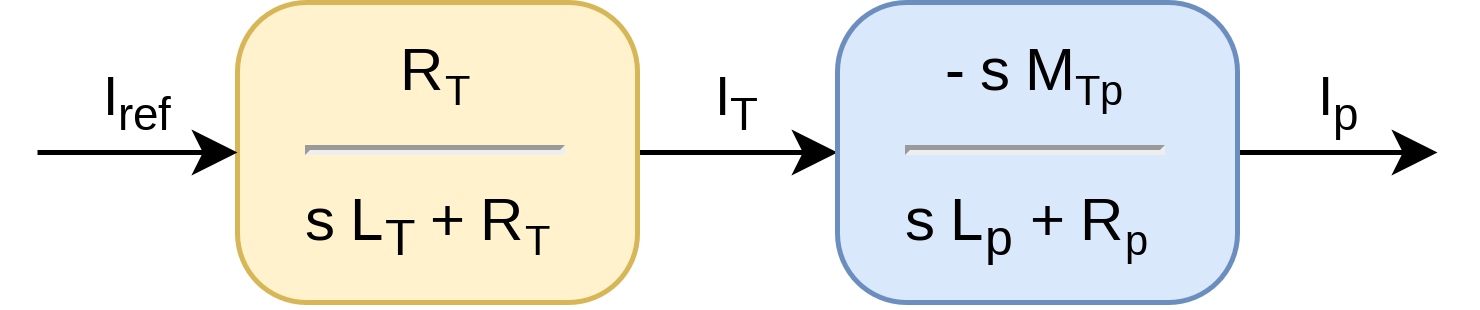
\includegraphics[width=1\textwidth]{Trasformatore/PlasmaCircuit-SchemaBlocchi.png}
\end{figure}\vspace{-6mm}
\noindent
Essendo il segno di uscita del segnale inverso rispetto al segnale d'ingresso, eliminiamo questo fastidio aggiungendo matematicamente un '$ - $' e a livello di prototipo invertendo i fili sul Secondario. Così facendo otteniamo come funzione di trasferimento complessiva:
\begin{empheq}[box=\mathCalc]{equation} \label{eq:FuncTrasfTotPos}
	P_{pos}(s) = -P(s) = \frac{s M_{Tp}}{( s L_p + R_p)(s L_T + R_T)} = \frac{-I_p(s)}{I_{ref}(s)}
\end{empheq}

\subsection{Misura del campo Elettrico del Plasma come indice per la Corrente} \label{sub:parametriMisurati}
Riprendendo l'equazione della corrente di Plasma \ref{eq:correntePlasmaDinamica}, abbiamo che il campo elettrico indotto sul Plasma, ovvero la $F_{em}$, dipende direttamente dallo stato della corrente di Plasma $I_p$.\\
Da essa abbiamo che per $I_p$ costanti, anche la $F_{em}$ è costante.\\
Nel caso del trasformatore si potrebbe fisicamente misurare la corrente di Plasma, simulata dalla corrente sul secondario, ma nel caso di un impianto reale, risulta evidente che è impossibile.\\
Proprio per questo, come descritto da \cite{MagneticDiagnostics},a pagina 12, si usa come indice di misura Tensione di giro $V_{loop}$ ($\Rightarrow F_{em}$ nel nostro esperimento).\\
Perciò il circuito reale usato nell'esperimento della tesi, comprensivo di misure è:
\begin{figure}[H] \label{fig:circuitoDiMisura}
	\centering
	\caption[Circuito reale di misura dell'esperimento]{Circuito di misura}
	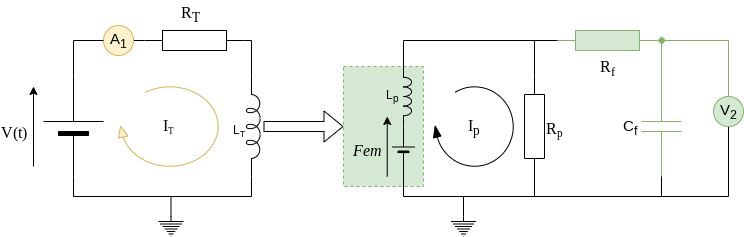
\includegraphics[width=1\textwidth]{Trasformatore/PlasmaCircuit-MisureCircuit.png}
\end{figure}

Abbiamo quindi, tra ingresso e uscite i parametri di:
\begin{itemize}
	\item $I_T$ misurata dal sensore di corrente $ A_1 $ \nameref{CurrentSense}.
	\item $F_{em}$ misura dal voltmetro $V_2$ (che è realizzata da un Pin analogico del \microControllore) e che rappresenta un indice per  la corrente $I_p$ quando essa è costante (eq \ref{eq:correntePlasmaDinamica}).
	\item $V(t)$ generata in base alla legge di controllo, e attuata mediante PWM (\cite{modulazionePWM}) dal driver di corrente \nameref{CurrentDriver}.
\end{itemize}


\newpage


\section{Trasduttore di Corrente}\label{CurrentSense}
Come già discusso precedentemente, l'obiettivo della tesi è di controllare la corrente sul secondario. In tale ottica la misura della corrente sul Primario potrebbe non essere una misura di interesse. Essendo però un lavoro di ricerca, si è preferito poter misurare la corrente effettivamente circolante nel Primario del trasformatore, così da poter meglio interpretare i dati misurati senza ambiguità.
\begin{figure}[H]
	\centering
	\caption[Sensore di Corrente \citefield{ACS770}{series}]{Sensore di Corrente}
	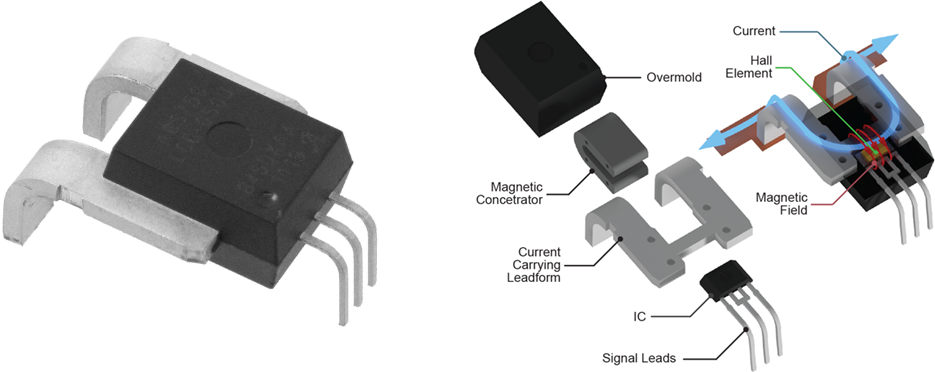
\includegraphics[width=1\textwidth]{ACS770/ACS770-Fig.png}
\end{figure}
%\vspace{-1cm}
\subsection{Sensore scelto}
Per misurare la corrente del primario, si è usato il sensore di Corrente \cite{ACS770}. La famiglia di sensori ha in generale le seguenti caratteristiche:
\begin{table}[H]
	\centering
	\label{tab:ACS770ParametriGenerali}
	\caption[\cite{ACS770}  Riassunto caratteristiche]{Riassunto caratteristiche}
	\begin{tabular}[t]{|l r|}
		\hline
		Bandwidth:                             & 120 kHz                               \\
		Output rise time :                     & 4.1 $ \mu s $                         \\
		Ultralow power loss:                   & 100 $ \mu \Omega $ Resistenza Interna \\
		Single supply operation                & 4.5 to 5.5 V                          \\
		Extremely stable output offset voltage &                                       \\
		\hline
	\end{tabular}
\end{table}
\noindent
In oltre, delle tante varianti esistenti, si è scelto di usare la \citefield{ACS770}{series}, le cui caratteristiche chiave sono:

\begin{table}[H]
	\centering
	\label{tab:ACS770ParametriParticolari}
	\caption[\citefield{ACS770}{series} Particolarità]{\citefield{ACS770}{series} Particolarità}
	\begin{tabular}[t]{|l r|}
		\hline
		Primary Sampled Current: & $\pm$ 100 A     \\
		Sensitivity Sens (Typ.)  & 20(mV/A)        \\
		Current Directionality   & Bidirectional   \\
		$T_{OP}$                 & –40 to 150 (°C) \\
		\hline
	\end{tabular}
	
\end{table}
\noindent
Le caratteristiche più importanti di questo trasduttore sono l'ampio margine di misura, e la robustezza alle variazioni di temperatura, che insieme rendono il dispositivo perfetto per misurare le energie dei nostri esperimenti attuali, e lo rendono \textit{future-proof} per esperimenti futuri quando si useranno energie superiori.

\subsection{Criticità}
Unico punto dolente, ma comune al tutti i sensori a effetto induttivo, è proprio il suo principio di funzionamento: essendo il sensore basato su un l'effetto Hall, ovvero una misura diretta del campo magnetico indotto dalla corrente nel conduttore, lo rende soggetto alle variazioni di campo magnetico prodotte propri dal Trasformatore Centrale, che nei suoi momenti di massimo flusso, genera ovviamente un campo magnetico non indifferente.
\begin{figure}[H]
	\centering
	\caption[Metodo di misura di corrente mediante effetto Hall]{Misura di corrente per effetto Hall}
	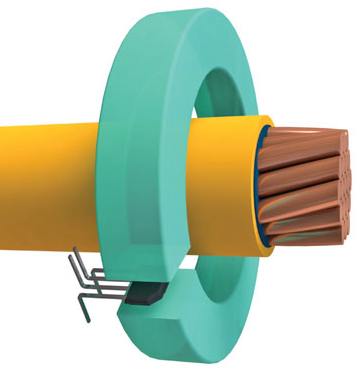
\includegraphics[width=0.5\textwidth]{ACS770/effettoHall.png}
\end{figure}
\newpage
\subsection{Funzionamento Interno}
\vspace{-5mm}
\begin{figure}[H]
	\centering
	\caption[\citefield{ACS770}{series} Schema a Blocchi]{Schema a Blocchi}
	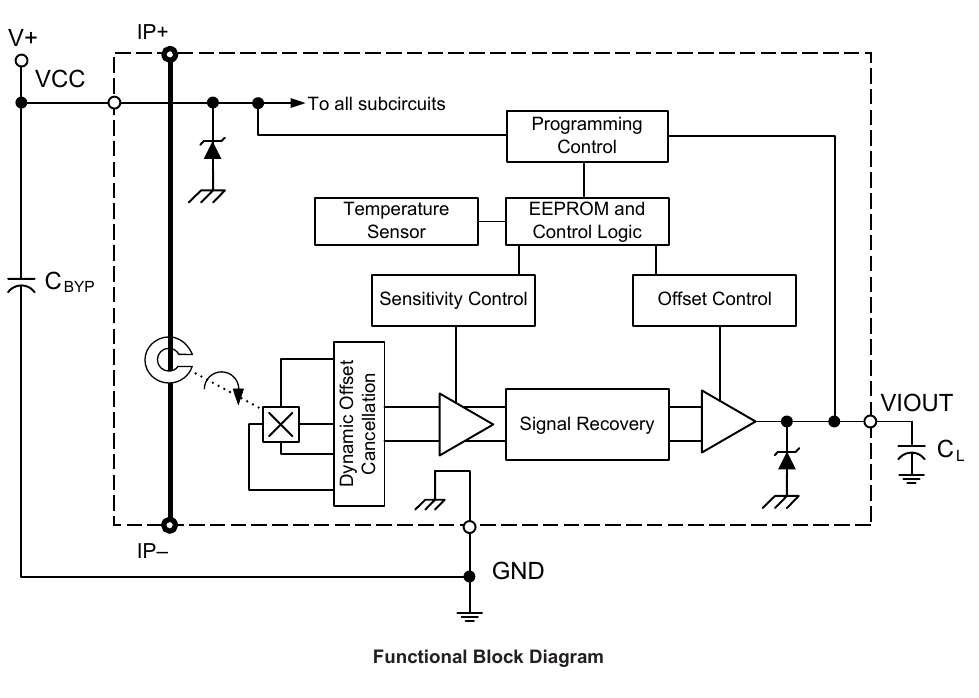
\includegraphics[width=1\textwidth]{ACS770/ACS770-SchemaBlocchi.png}
\end{figure}
\noindent
Tra le caratteristiche chiave dell'\cite{ACS770}, troviamo il disaccoppiamento fisico tra la corrente da misurare e il circuito di misura (ben visibile nello schema a blocchi). Questa caratteristica chiave, garantisce la salvaguardia del circuito logico a valle, dai possibili eventi catastrofici a monte.\\
Esso è in oltre fornito di sensori di temperatura e sistemi di \textit{Signal Recovery} che permettono all'Hardware stesso di compensare parzialmente \nonLinearita termiche della misura per effetto Hall, ottenendo un output assimilabile a un segnale lineare:
\newpage
\begin{figure}[H]
	\centering
	\caption[\citefield{ACS770}{series} Sensibilità rispetto Temperatura]{Sensibilità}
	\includegraphics[width=0.65\textwidth]{ACS770/ACS770-Sensibilità.png}
\end{figure}
\vspace{-5mm}
\noindent
Come si può vedere dal grafico, gli errori sono tanto più marcati quanto maggiore è la corrente da misurare ed in oltre questo errore ha una forte dipendenza dalla temperature dell'esperimento:\\\vspace{-12mm}
\begin{figure}[H]
	\centering
	\caption[\citefield{ACS770}{series} \nonLinearita]{Temperatura/NonLinearità}
	\vspace{1mm}
	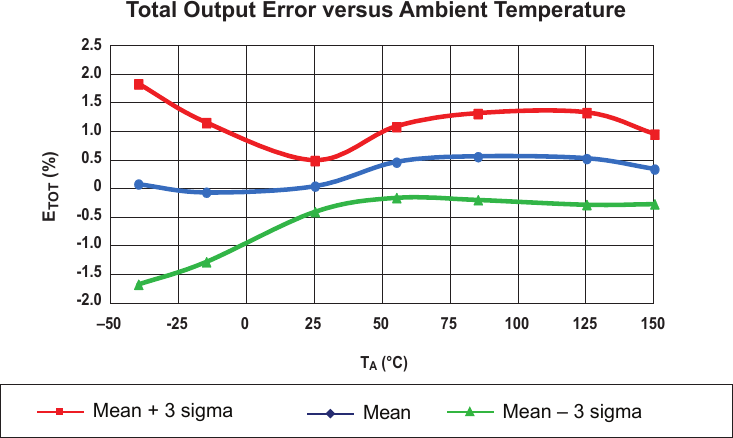
\includegraphics[width=0.9\textwidth]{ACS770/ACS770-NonLin.png}
\end{figure}\vspace{-6mm}

\noindent
Il quale però non è mai, neanche negli esperimenti più sfortunati, superiore al $\pm2\%$.\\
Anzi, alle temperature $\approx$ 25°, si mantiene contenuto tra $\pm0.5\%$.

\newpage

\subsection{Connessione elettrica}

La connessione del sensore è particolarmente semplice, richiedendo esternamente solo un alimentazione stabilizzata e portando subito in uscita la misura di corrente sotto forma di tensione.
\begin{figure}[H]
	\centering
	\caption[\citefield{ACS770}{series} Schema di collegamento dal Datasheet]{Collegamento dal Datasheet}
	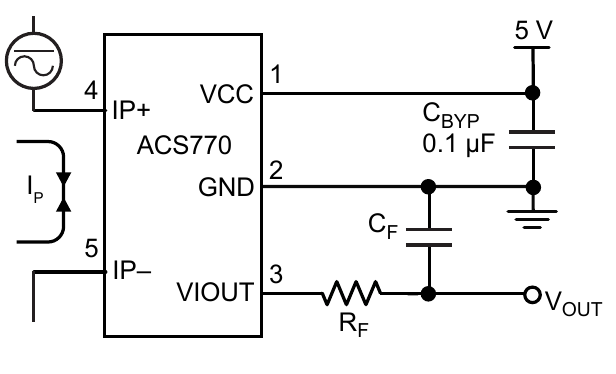
\includegraphics[width=0.85\textwidth]{ACS770/ACS770-Schema.png}
\end{figure} \vspace{-8mm}
\noindent
Rispetto allo schema proposto dal datasheet, però, si è deciso di omettere il filtro passa-basso sulla \textbf{VIOUT}, questa scelta è stata presa per minimizzare il più possibile ritardi di misura della corrente istantanea desiderabile poiché le dinamiche del sistema sul secondario, come visto, sono di tipo derivativo, e quindi estremamente rapide.\\
Questa scelta è stato possibile prenderla poiché la corrente per alimentare l'esperimento proviene da una batteria con un alta capacità di scarica istantanea (fino a 1000A), da cui l'assenza di disturbi sul segnale di corrente e la possibilità di prendere questa scelta.

\subsection{Dalla misura alla corrente}
Il trasduttore è basato sull'effetto Hall, il quale permette di misurare una corrente attraverso il campo magnetico che crea, e riporta questa misura sotto sotto forma di tensione.\\
I sensori della famiglia \cite{ACS770} propongono vari modelli che differiscono tra loro principalmente per la \textbf{Sensibilità} di misura e la lettura di corrente \textit{Bi-direzionale} o \textit{Mono-direzionale} , in funzione della scala di misura che si vuole avere e della presenza di corrente alternata o continua.
Per i nostri scopi abbiamo preso il modello: '\citefield{ACS770}{series}', di cui i parametri sono riportati in tabella \ref{tab:ACS770ParametriParticolari}.\\
Usando la sensibilità riportata in tabella, abbiamo che la formula di conversione per ottenere la corrente letta è:
 \begin{center}
 	{\large $I_{read} = \frac{V_{Read}[V]}{V_{sense}[V/A]}$ }
\end{center}


\paragraph{Rimozione Offset}
Essendo però l'ACS770 ad alimentazione singola (0--5V), ma la corrente misurabile \textbf{Bi-Direzionale}, sorge la necessità di spostare il riferimento della corrente nulla ad una tensione superiore allo 0V.\\
Il datasheet riporta che $V_{offset} = \frac{Vcc}{2}\approx$ 2.5V. Da cui deriva che la vera misura di corrente è:

{\large
\begin{empheq}[box=\mathCalc]{equation}\label{eq:Iread}
	I_{read} = \frac{V_{Read}-V_{offset}}{V_{sense}} \frac{[V]}{[V/A]}
\end{empheq}
}
\noindent
Al fine di poter misurare l'offset effettivo, durante il set-up viene eseguito a esperimento fermo una misura dell'offset attuale, usando la \nameref{lst:offsetCalc}.\\
Il risultato della computazione, oltre ad essere usato nel controllo è inviato al computer per la post elaborazione dei dati nei grafici.

\paragraph{Analisi Sensibilità}
Usando nell'esperimento un ADC a 10Bit con tensione di riferimento a 5V, abbiamo che la massima sensibilità del \microC, ovvero il suo bit meno significativo è pari a:
%\vspace{-5mm}
\begin{empheq}[box=\mathResult]{equation} \label{result:Vstep}
	V_{step}=\frac{Vcc}{2^{10}-1} = 4,887mV
\end{empheq}
\noindent
Il che equivale a una \textbf{Sensibilità di Corrente} del $\mu$Controllore pari a:
%\vspace{-5mm}
\begin{empheq}[box=\mathResult]{equation} \label{result:Istep}
	I_{step} =\frac{ V_{step}}{V_{sense}} = 244,379 mA
\end{empheq}

\newpage

\section{Driver di Corrente - IBT-2}\label{CurrentDriver}
Per l'attuazione del controllo di corrente nella bobina primaria del trasformatore, è stato usato il driver di corrente \cite{IBT-2} .


\begin{figure}[H]
	\centering
	\caption[Driver Motori IBT-2 TopView \& PinOut]{IBT-2 TopView.}
	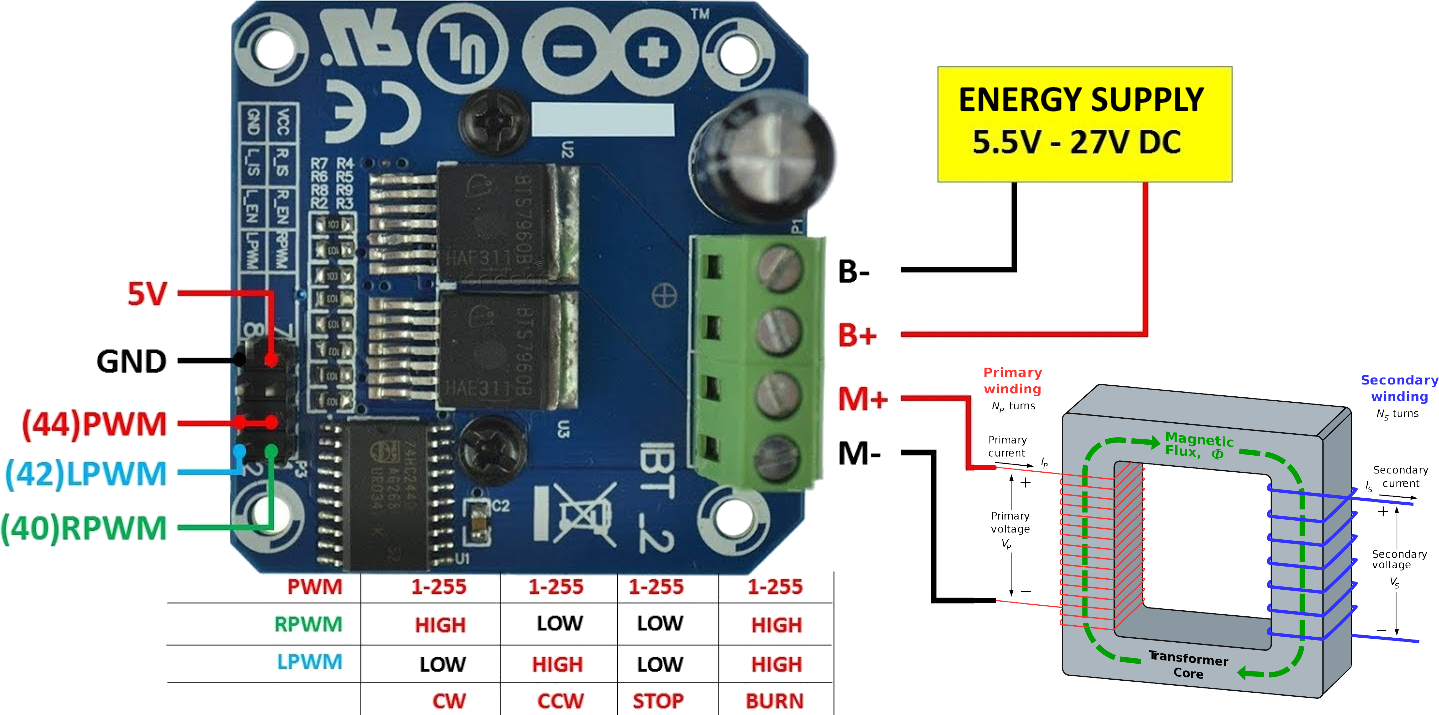
\includegraphics[width=1\textwidth]{IBT-2/TopView.png}
\end{figure}

\noindent
Esso non è un comune Ponte-H integrato: per poter gestire potenze superiori è stato costruito usando 2 Half-Bridge (\cite{BTS7960b}) collegati assieme mediante una opportuna logica per ricreare un normale Ponte-H.\\
Questa scheda in particola ha prestazioni interessanti per gli scopi di questa tesi, i principali sono elencati di seguito:\vspace{-8mm}
\begin{table}[H]
	\centering
	\caption[IBT-2 Specifiche]{IBT-2 Specifiche}
	\begin{tabular}[t]{|l r|}
		\hline
		Power Input Voltage:                                     & 6 -- 27 V \\
		Peak current:                                            & 43 A      \\
		Massima Frequenza di PWM:                                & 25 kHz    \\
		Protezione Sovra Tensioni                                &           \\
		Disaccoppiamento Ingresso di Potenza/Logica di controllo &           \\
		\hline
	\end{tabular}
\end{table}\vspace{-4mm}
\noindent
Di particolare interesse per l'esperimento è proprio la corrente di picco gestibile:
avendo le dinamiche del sistema tempi inferiori ai 5 secondi, poter reggere correnti di picco così elevate rende
la scheda perfetta per i nostri scopi.

\newpage
\subsection{Schema Elettrico}
Al suo interno il driver è composto da 2 Half-Bridge \cite{BTS7960b}, connesse secondo lo schema:
\begin{figure}[H]
	\centering
	\caption[IBT-2 Schema Elettrico]{IBT-2 Schema Elettrico}
	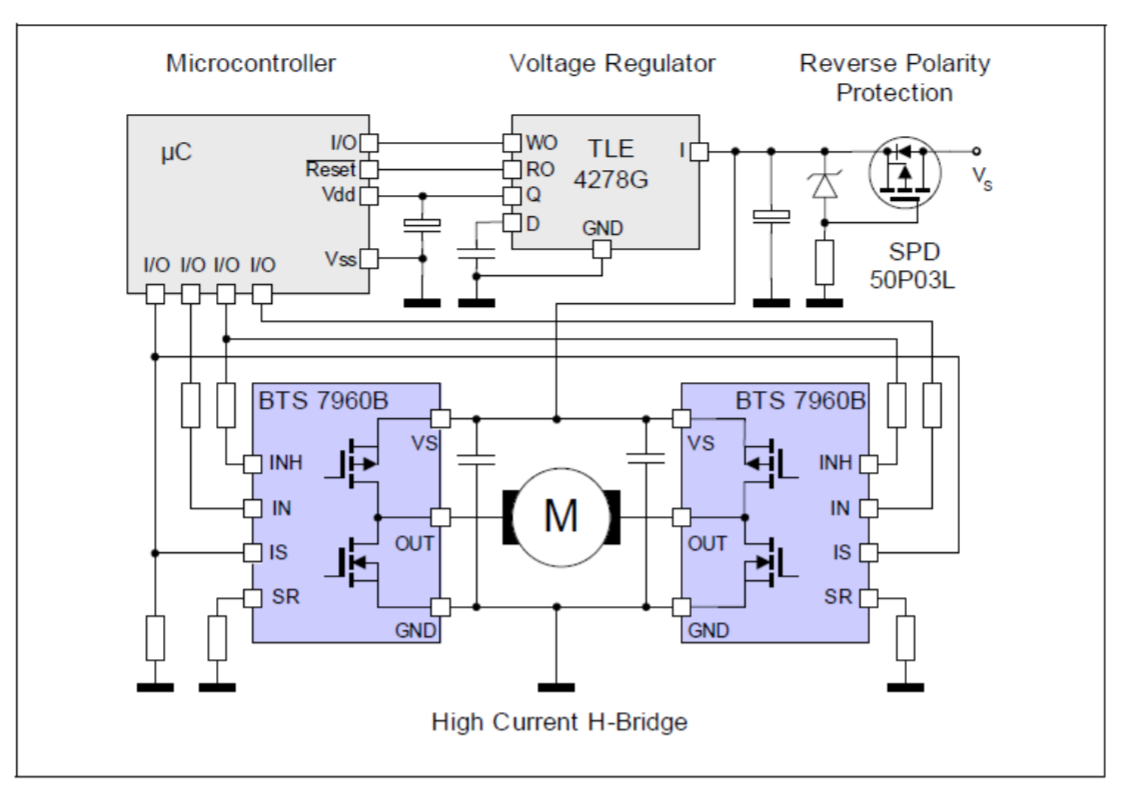
\includegraphics[height=0.5\textheight]{IBT-2/elettricScheme.png}
\end{figure}\vspace{-5mm}

\noindent
Il \microC è protetto dal carico connesso all'interno del \citefield{BTS7960b}{series}, lasciando al \microC solo il compito di controllare i segnali che commutano lo stato dei 2 Half-Bridge.
\newpage
\subsection{Connessione di Controllo}
Il driver permette 2 modalità di funzionamento:
\begin{description}
	\item[Doppio PWM] Modalità operativa che richiede l'uso di 2 PWM\\
	      Ciascun PWM controlla uno dei 2 Half-Bridge, e per evitare di bruciare i driver devono essere controllati singolarmente, il vantaggio di questa configurazione è la possibilità di usare 2 frequenze di controllo diverse.
	\item[Singolo PWM] Modalità operativa classica di un normale Ponte-H\\
	      In questa modalità, la porta nand presente sulla scheda attua la logica di controllo opportuna per governare i 2 Half-Brige come fossero un normale Ponte-H.
\end{description}

\noindent
Per il nostro esperimento si è scelto di usare il collegamento \textbf{\underline{Singolo PWM}} così da evitare spiacevoli sorprese e avere il PWM di controllo sempre sincronizzato.	

\newpage
\subsection{Benchmark del Driver}
Il driver sulla carta ha buone prestazioni, dal datasheet non risaltano \nonLinearita, esse invece sono presenti e per farle risaltare si sono effettuati 2 segnali di input:
\begin{enumerate}
	\item \nameref{lst:ondaTriangloare} \vspace{-3mm}
	      \begin{figure}[H]
		      \caption[Esperimento con Onda Triangolare]{Onda Triangolare}
		      \centering
		      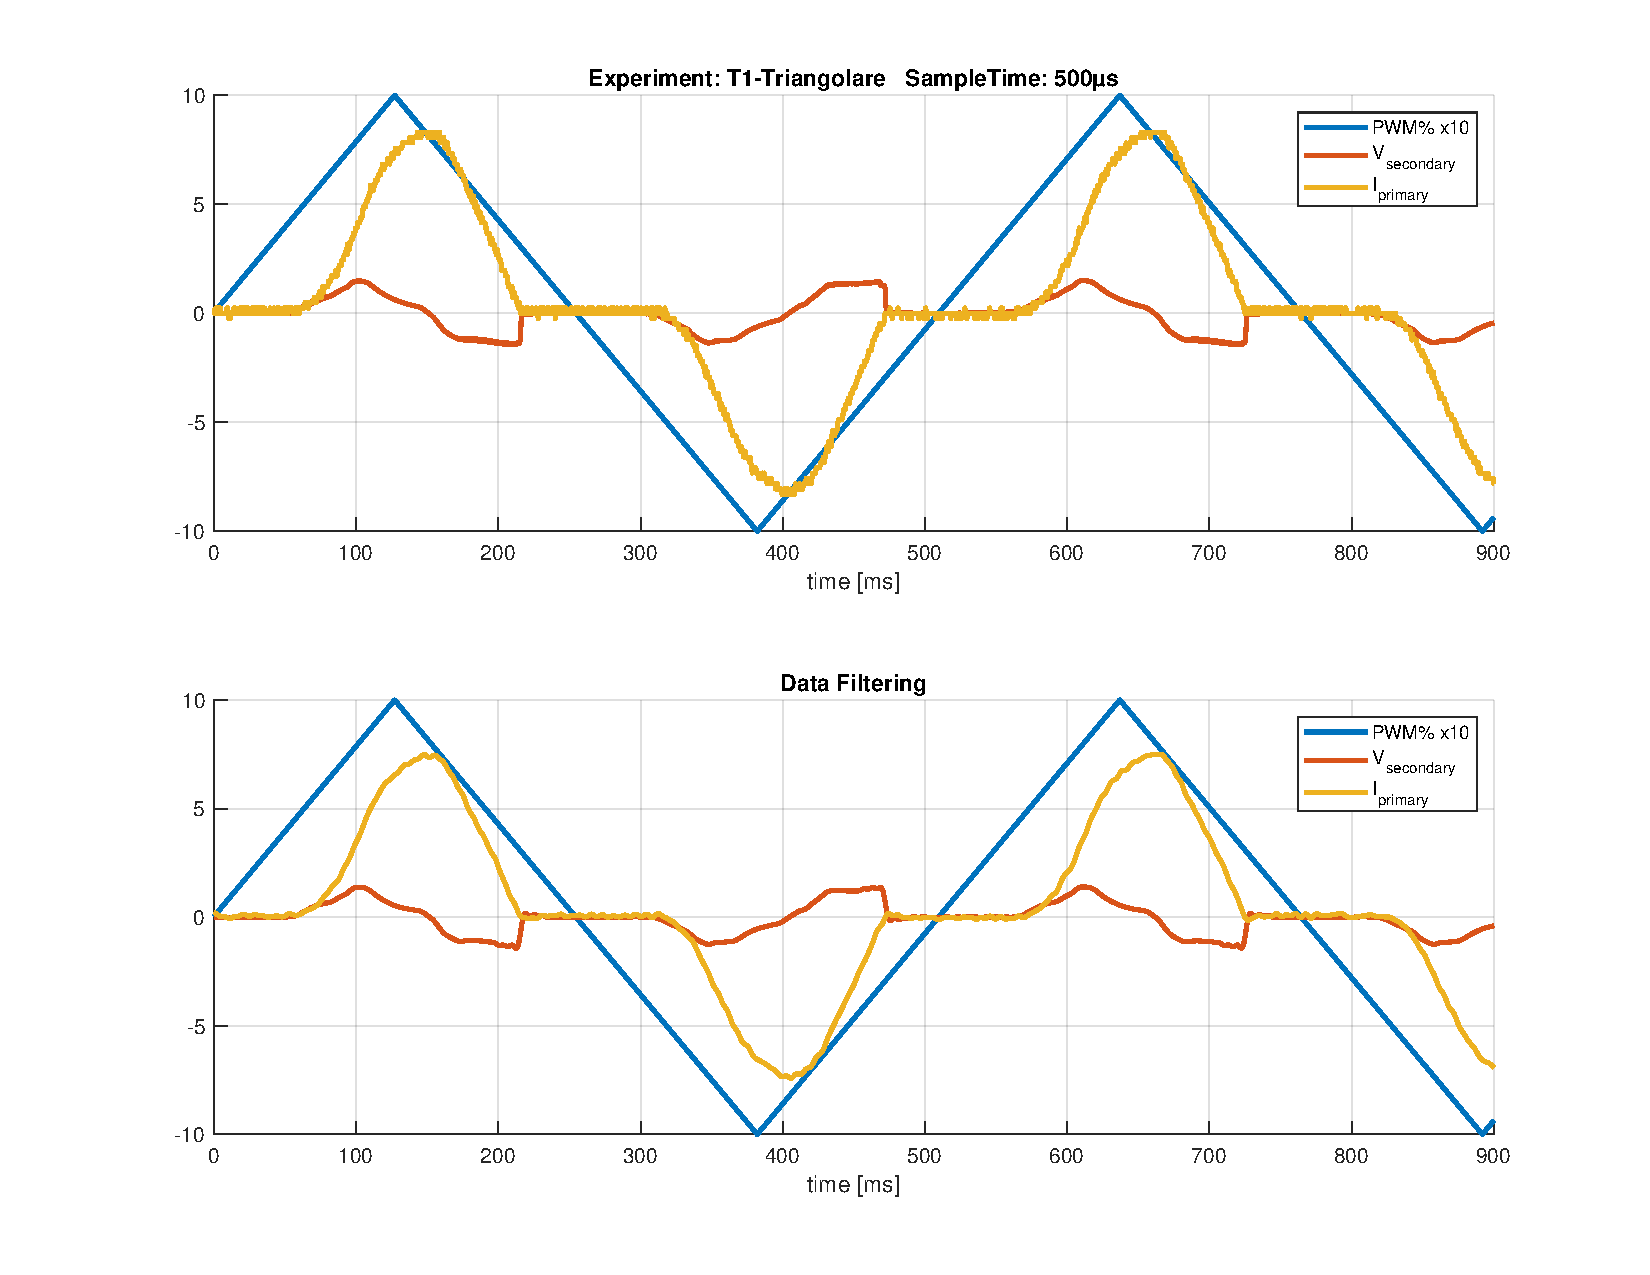
\includegraphics[height=0.5\textheight]{IBT-2/T1-Triangolare.pdf}
	      \end{figure}\vspace{-10mm}
	      \paragraph{Dead-Zone Inferiore} L'onda triangolare si presta bene per far risaltare la problematica della Dead-Zone Inferiore, infatti in tutti gli intorni in cui il segnale passa per 0, è possibile vedere come tanto la corrente quanto la tensione sul secondario non vari minimamente, indice evidente dell'assenza di corrente e quindi della presenza della \textbf{Dead-Zone}.\\
	      Per calcolare la soglia di \textbf{Dead-Zone Inferiore} è sufficiente vedere il primo valore di PWM  per cui il sistema risponde dopo il passaggio per 0.      
	      \newpage
	\item \nameref{lst:ondaTrapezoidale}  \vspace{-3mm}
	      \begin{figure}[H]
		      \centering
		      \caption[Esperimento con Onda Trapezoidale (\textit{Rapid Shot})]{Onda Trapezoidale (\textit{Rapid Shot})}
		      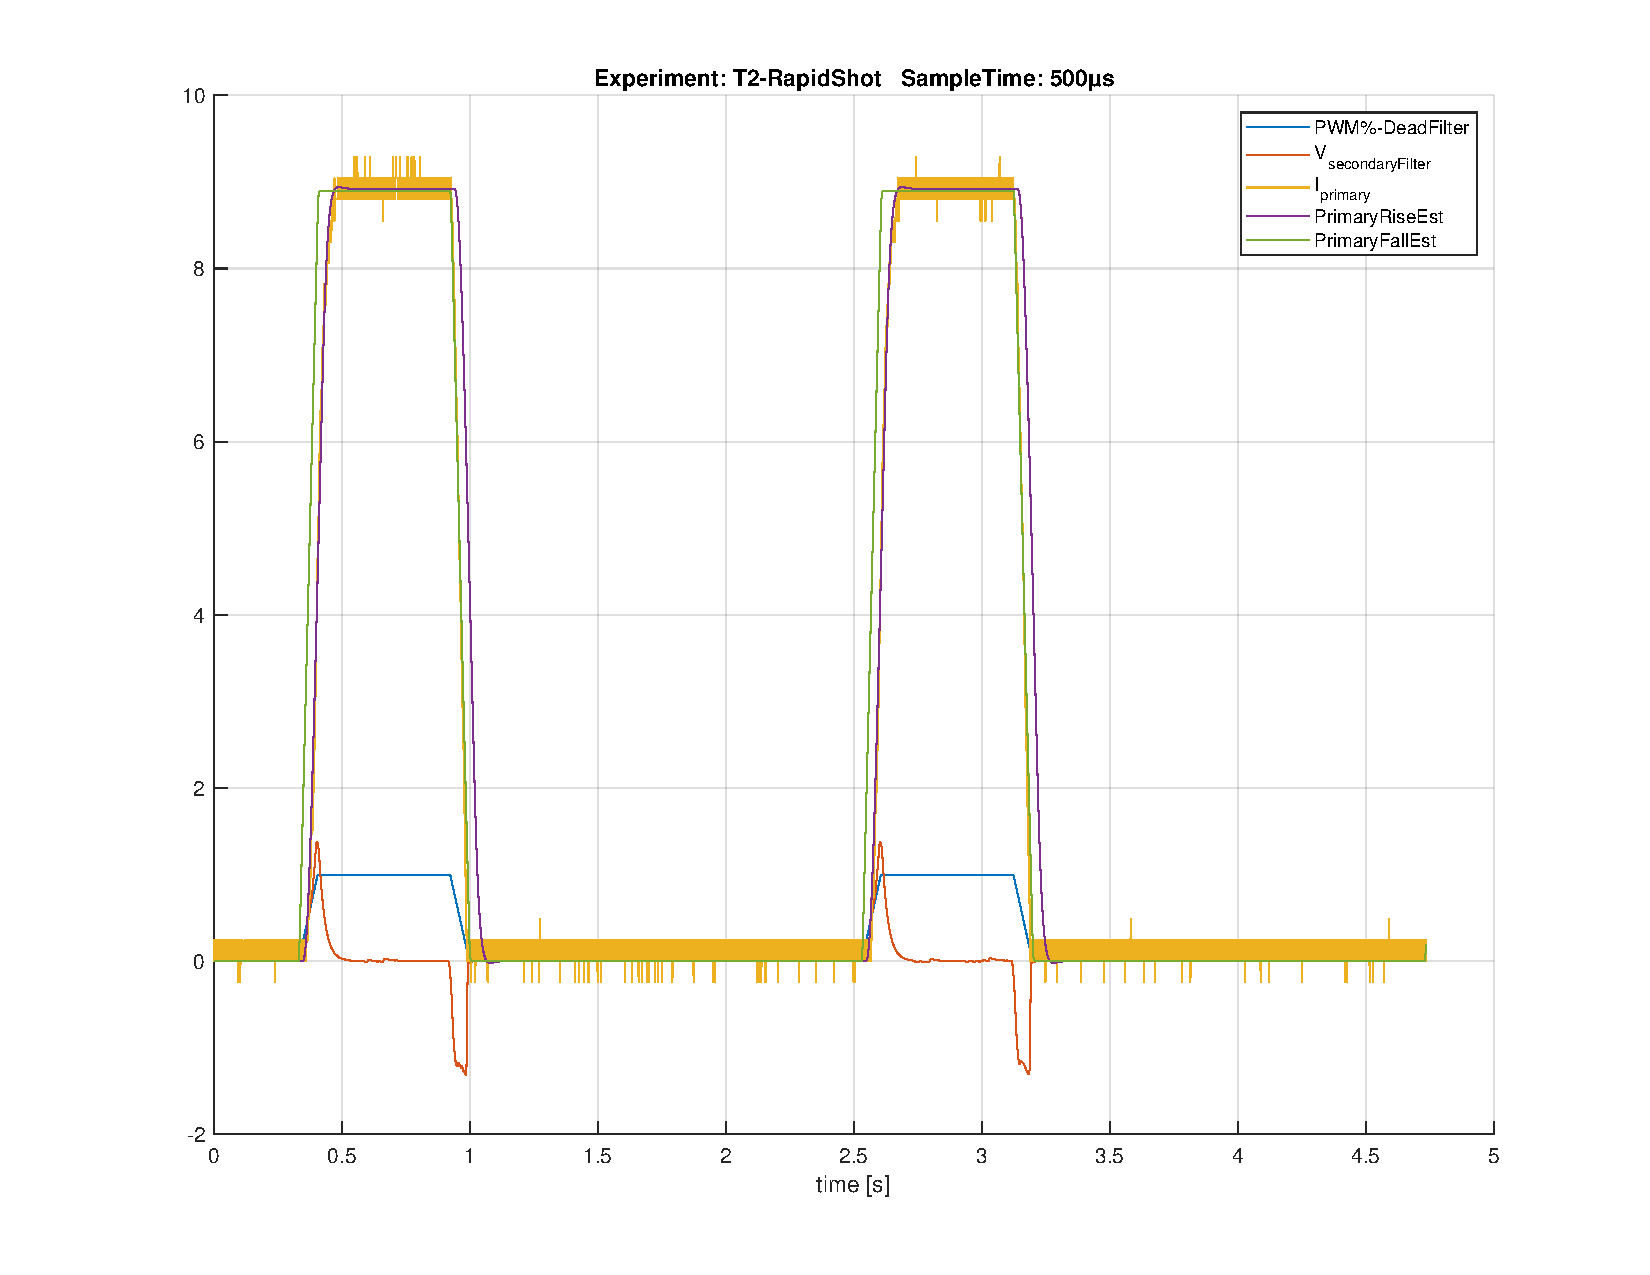
\includegraphics[height=0.5\textheight]{IBT-2/T2-RapidShot.pdf}
	      \end{figure}  \vspace{-15mm}
	      \paragraph{Dead-Zone Superiore} Usando il segnale \textit{Rapid Shot} mettiamo in evidenza la presenza della \textit{Dead-Zone Superiore}, visibile sotto forma di ritardo di attuazione nella rampa di discesa.\\
	      Il ritardo è pari a circa 20ms {\small \textit{(guarda 900ms)}}, e come detto è causato dalla seconda Dead-Zone presente nel driver.
\end{enumerate}
\noindent
Il driver soffre di questi problemi poichè per i Duty-Cycle \textit{Alti} e \textit{Bassi} nel PWM, prima uno e poi l'altro Half-Bridge, non fa in tempo a commutare che il segnale ha nuovamente cambiato valore, causando di fatto questa assenza di attuazione e quindi la Dead-Zone. Sapendo della presenza di queste 2 Dead-Zone, risaliamo ai loro valori di soglia andando a vedere l'inizio della risposta del secondario per entrambi i fronti:\vspace{-4mm}
\begin{table}[H]
	\centering
	\caption[Fasce della Dead-Zone]{Fasce della Dead-Zone}
	\begin{tabular}[t]{||c r||}
		\hline
		Dead-Zone Superiore & $\pm$ 210 PWM  \\
		Dead-Zone Inferiore & $\pm$ 120  PWM \\
		\hline
	\end{tabular}
\end{table}